%%%%%%%%%%%%%%%%%%%%%%%%%%%%%%%%%%%%%%%%%%%%%%%%%%%%%%%%%%%%%%%%%%%%%%%%%%%%%%%%
% placeholder.tex
%
% Modelo de arquivo para uso com a classe uvvTeX2, para a formatação de
% trabalhos acadêmicos na Universidade Vila Velha (UVV) (https://www.uvv.br).
%
% Para maiores informações, visite:
%    https://github.com/uvv-computacao/uvvtex2
%
% Este placedholder apenas indica uma forma comum de incluir imagens em seu
% trabalho. Use o código a seguir como base e consulte a documentação do
% LaTeX para maiores informações.
%%%%%%%%%%%%%%%%%%%%%%%%%%%%%%%%%%%%%%%%%%%%%%%%%%%%%%%%%%%%%%%%%%%%%%%%%%%%%%%%

\begin{figure}[htbp]
\centering
\caption{Arquitetura da VPC com container acessando a internet via NAT Gateway}
\label{fig:vpc-simples}
\fbox{
   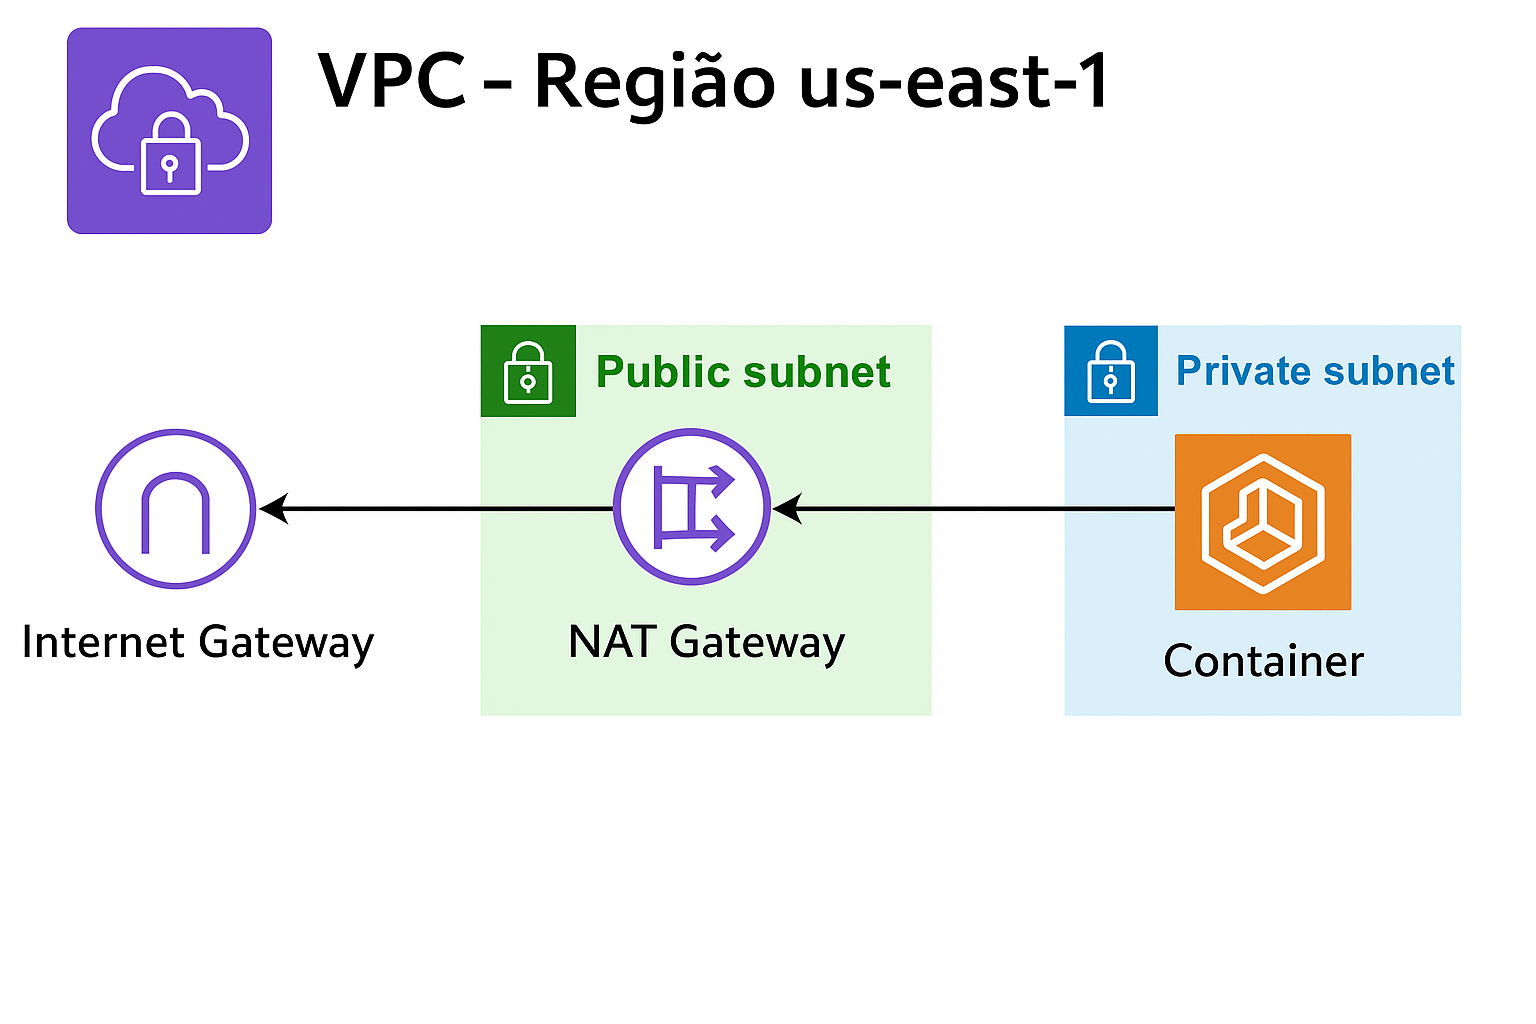
\includegraphics[scale=0.3]{tcc1/imagens/vpc-simples.png}
}
\legend{Representação da infraestrutura configurada na AWS: o container, alocado em uma subnet privada, acessa a internet por meio de um NAT Gateway posicionado em uma subnet pública.}
\end{figure}

\begin{figure}[H]
\centering
\caption{Arquitetura geral do ambiente na AWS}
\label{fig:arquitetura-geral}
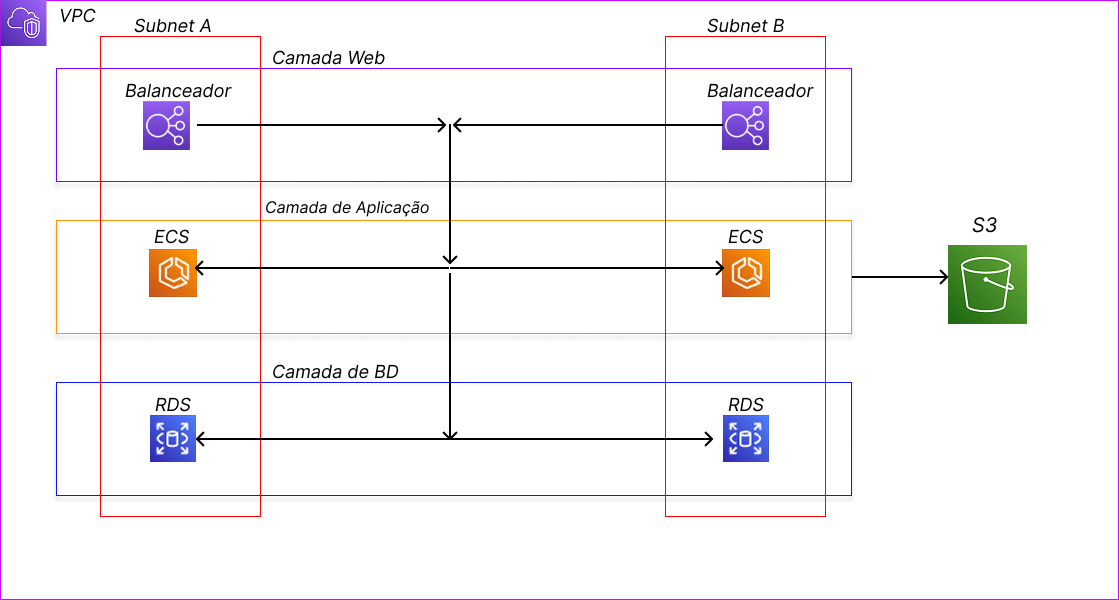
\includegraphics[scale=0.45]{tcc1/imagens/arquitetura.png}
\legend{Visão em camadas da infraestrutura: balanceamento, aplicação e banco de dados, com distribuição entre duas sub-redes em Zonas de Disponibilidade distintas.}
\end{figure}
